
\documentclass{article}
% pre\'ambulo

\usepackage{lmodern}
\usepackage[T1]{fontenc}
\usepackage[spanish,activeacute]{babel}
\usepackage{mathtools}
\usepackage{graphicx}
\graphicspath{ {latex/} }

\title{Tarea 01}
\author{Nestor Semer V\'azquez Cordero}
\date{14 de Agosto del a\~no 2019}

\begin{document}
% cuerpo del documento

\maketitle

\section{Definici\'on del problema}

Dar el clima en tiempo real de dos localidades dadas su latitud y longitud, 
usando un web service para poder realizar las multiples peticiones que se requieren.

\section{Analisis del problema}
Realizar 
\section{Seccion de la mejor alternativa}

Se utilizar\'a el lenguaje de programacio\'n python ya que es un lenguaje lenguaje de alto nivel, 
debido a eso la sintaxis es sencilla, adem\'as  hay librerias que facilitan el trabajo al realizar las peticiones y obtener el archivo json.

\section{Diagrama de flujo }
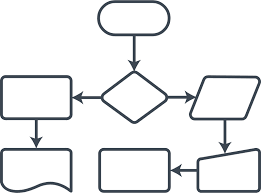
\includegraphics{diagrama}
\section{Pensando en el futuro}

\end{document}
